%========ANÁLISIS DE FACTIBILIDAD
\section{Analísis de Factibilidad}
\paragraph{Introducción}
Para el desarrollo de aplicaciones moviles se encuentran diferentes herramientas para llevarlas acabo dentro de las cuales destacan :
Librerias ,Lenguajes de programacion o Arquitecturas.
Por lo cual se debe de definir un modelo el cual tenga un nivel alto de interoperabilidad entre los componentes del sitema.


\section{Factibilidad Tecnica}
La utilización de un analísis de factibilidad tecnica nos permite recolectar información necesaria sobre los recursos de software , hardware , conocimientos y habilidades de los cuales se puede hacer uso dentro del desarrollo e implementación del trabajo, no obstante el analísis de factibilidad tambien nos permite definir con mayor claridad los requerimientos tecnológicos que deben de ser utilizados para que el desarrollo tenga el menor indice de riesgo posible.


\paragraph{1.-Tipos de aplicaciones:}

Existen 3 tipos diferentes de aplicaciones movil , los factores en los cuales se basan para clasificarlas dependen de la funcionalidad y la forma en que seran realizadas. Los puntos mas destacables a la hora de una eleccion de aplicacion movil es sin duda la red de internet , ya que las aplicaciones moviles pueden trabajar con red de internet o se pueden ejecutar sin problemas desde el dispositivo sin contar con una red de internet.
A continuacion se explicara en una breve tabla las ventajas y desventajas que estas tienen:
\begin{table}[h!]
\begin{tabular}{|p{2.5cm}|p{5cm}|p{4cm}|p{4cm}|}
\hline
\textbf{Tipos de aplicaciones moviles}&\textbf{Descripción}& \textbf{Ventajas}& \textbf{Desventajas}\\
\hline
\hline
AppsNativas& Una aplicación nativa, se caracteriza por haber sido desarrollada especialmente para un lenguaje de programación.&
\begin{UClist}
		\UCli Notificaciones push
		\UCli Rapidez de navegación
		\UCli Uso complejo del hardware
		\UCli Facil Manejo
		\UCli Diseño y desarrollo Personalizado
		\UCli No necesitan conexión a internet
\end{UClist} & \begin{UClist}

\UCli Mayor tiempo de desarrollo
\UCli Precio mas elevado
\end{UClist} \\
\hline
\hline
WebApss&Este tipo de aplicaciones se caracterizan por estar desarrolladas en lenguajes de programación propias de la web, como HTML, CSS o Javascript.
& 	\begin{UClist}
		\UCli Multiplataformas
		\UCli Responsive Desing
	\end{UClist} &
	\begin{UClist}
		\UCli No requieren instalación por lo tanto no estaran disponibles en las tiendas de aplicaciones (Play Store , Apple Store).
		\UCli El diseño es totalmente web , "Responsive Desing" lo adapta a una plataforma movil.
	\end{UClist} \\
\hline
\hline
WebApps Nativas & Las Webapps Nativas es una combinacion de Webapps y appsnativas las cuales tienen la mayor parte de su estructura realiza en lenguajes de programación de la web , no dejando aun lado la parte nativa del movil. & 
	\begin{UClist}
		\UCli Multiplataforma
		\UCli Herramientas de lenguajes nativos
	\end{UClist} &
	\begin{UClist}
		\UCli Costo Elevado
	\end{UClist} \\
\hline



\end{tabular}
\caption{Tipos de aplicaciones.}
\label{disenoEstructura:TipoApp}
\end{table}

Para este trabajo terminal se hara uso total de las aplicaciones nativas ya que estas se centran en un solo lenguaje de programación ayudando asi a reducir considerablemente el tiempo de producción de la aplicación movil.



\paragraph{2. Software :}
En el mundo del desarrollo para móviles actualmente se dispone de muchas opciones para ello se debe tomar en cuenta los lenguajes y herramientas nativos de cada plataforma.Para ello se hizo un analisis de las herramientas que estan disponibles para la realización de aplicaciones moviles.

\begin{table}[h!]
\begin{tabular}{|p{3cm}|p{3.5cm}|p{3cm}|p{3cm}|p{3cm}|}
\hline
\textbf{Herramienta}&\textbf{Ventajas}& \textbf{Desventajas}& \textbf{Lenguaje Utilizado} & \textbf{Tipo de Herramienta} \\
Xamarin & 	\begin{UClist}
				\UCli Basada en lenguaje mas populares
				\UCli Es universal para las diferentes plataformas
			\end{UClist} &
							\begin{UClist}
								\UCli Mayor tiempo de desarrollo
							\end{UClist} & C\# , .NET & Multiplataforma compilado a nativo \\
\hline
\hline
AndroiStudio & 	\begin{UClist}
					\UCli Compilación rapida
					\UCli Ejecución de aplicación en tiempo real
					\UCli Ejecución de aplicación directamente desde el movil
					\UCli Renderizado en tiempo real
					\UCli Uso de parametros tools
				\end{UClist} &
								\begin{UClist}
									\UCli Los requisitos minimos de hardware son elevados.
									\UCli Se requiere una computadora de gama alta
								\end{UClist} & Android & Nativo \\
\hline
\hline
Swift & \begin{UClist}
			\UCli Proceso de desarrollo rapido.
			\UCli Escalable al producto y al equipo.
			\UCli Seguridad y rendimiento.
			\UCli Disminución de la huella de memoria
		\end{UClist} & 
						\begin{UClist}
							\UCli Lenguaje joven.
							\UCli Interoperabilidad con herramientas de terceros e IDE.
							\UCli Falta de soporte para versiones anteriores
						\end{UClist} & IOS & Nativo \\
\hline


\end{tabular}
\caption{IDE}
\label{disenoEstructura:IDE}
\end{table}

Despues de el analísis correspondiente se ha concluido que android studio es la mejor herramienta para poder realizar la aplicación movil
ya que cuenta con uno de los mejores emuladores para realizar las pruebas correspondientes a la etapa de testing.

\paragraph{3. Sistema Operativo} 
Debido al desarrollo a una aplicación nativa , se hara uso de un sistema operativo en especial para que asi al momento de generar la implementación correspondiente no se obtenga fallos de compatibilidad con el sistema operativo . En la tabla \ref{disenoEstructura:SO} se muestra los sistemas operativos como tambien las versiones que serán evaluados para determinar cual se debe de utilizar.

\begin{table}[htbp]
\begin{tabular}{|p{3cm}|p{12cm}|}
\hline
\textbf{Nombre}&\textbf{Descripción}\\
\hline
\hline
GNU/Linux & El sistema operativo Linux es considera un sistema operativo libre tipo Unix , del cual destacan sus caracteristicas como la multiplataforma, multiusuario y multitareas. Ademas el sistema operativo Linux es considerado como uno de los sitemas operativos mayormente soportados por la alta iteroperabilidad que tiene con las principales plataformas informaticas.  \\
\hline
\hline
Windows 8.1® & Windows 8.1 ® perteneciente a la gran cadena de microsoft es una actualización al antiguo windows 8® . El cual te permite sincronizar mas configuraciones entre dispositivos , dentro de las configuraciones que mas destacan es la posibilidad de poder configurar la pantalla de inicio , configuración de teclado y raton por medio de bluetooth . Todo esto como parte de la expansión de configuracion PC.\\
\hline
\hline
Windows 10® & Windows 10® Es considerado el ultimo sistema operativo desarrollado por Microsoft® hasta la fecha actual , este sistema operativo pertenece a la familia de sistemas operativos NT. Dentro de los aspectos mas destacables que poseé este sistema operativo es la capacidad de tener una mejor armonización entre usuario y funcionalidad , ademas de corregir las deficiencias en las interfaces anteriores que se vienen presentando desde la presentacion de Windows 8® en el mercado   \\
\hline
\hline
Mojave® & La franquicia Apple ® tiene dentro de su mercado de ordenadores la ultima actualización conocida como Mojave que quita extensiones de aplicaciones que esten desarrolladas a 32 bits , esta actualizacioón presenta mejoras en la interfaz grafica para una mejor experiencia del usuario .  \\
\hline
\end{tabular}
\caption{SO}
\label{disenoEstructura:SO}
\end{table}

Una vez terminado el analísis se concluyo que se hara uso del sistema operativo mas actualizado enfocado a un mejor rendimiento de la aplicación web durante el desarrollo e implementación del mismo por lo cual se utilizara el sistema operativo Windows 10®.





\paragraph{4. Lenguaje de Programación} 
Para el desarrollo de aplicaciones movil, se manejan lenguajes  que son capaces de  ser interpretados por la mayoria de dispositivos moviles android el cual da la lógica a la aplicación.Existen una gran variedad de librerías las cuales facilitan el desarrollo movil.Para ello se realizo el siguiente analísis y asi poder elegir el lenguaje correspondiente.

\begin{table}[htbp]
\begin{tabular}{|p{3cm}|p{12cm}|}
\hline
\textbf{Nombre}&\textbf{Descripción}\\
\hline
\hline
C & El lenguaje de programación C es un lenguaje de medio nivel debido a los tipos de datos estaticos que utiliza por lo cual se encuentra debilmente tipificado ; es considerado lenguaje de medio nivel por que disponde de estructuras tipicas de los lenguajes de alto nivel , pero , asu vez, disponen de construcciones del lenguaje que permiten un control a muy bajo nivel. \\
\hline
\hline
Ensamblador & Este lenguaje es considerado de bajo nivel. Esta creado por conjuntos de mnemónicos que representan instruciones basicas para las computadoras , microprocesadores y microcontroladores. Este representa el codigo maquina especifico para cada arquitectura por medio del uso simbolico de los codigos de maquina binarias.\\
\hline
\hline
Java & Java es un lenguaje orientado a objetos con un proposito general . Este lenguaje fue diseñado para disminuir la dependencias de implementación ,  la intención de esto es permitir que los desarrolladores del programa escriban el codigo una vez y sea posible ejecutarlo en cualquier dispositivo , esto quiere decir que el codigo que es ejecutado en una plataforma no tiene que ser recompilado para que pueda ser utilizado en otra . \\
\hline

\end{tabular}
\caption{Lenguaje}
\label{disenoEstructura:Lenguaje}
\end{table}
Debido a la naturaleza de la presente aplicación movil , Se ha seleccionado el lenguaje de programacion Java para el desarrollo de la misma , ya que este se considera mas consistente en tanto a dependencias de implementación , por otro lado , Java es considerado un lenguaje orientado a objetos por lo cual nos permite trabajar de manera simultanea con el IDE seleccionado (AndroidStudio).

\paragraph{5. Sistema Gestor de Bases de Datos} 
Dentro de la aplicación debemos de seleccionar el mejor gestor de bases de datos para el almacenamiento de los mismos , para ello se necesita una solución con capacidad de soportar multiples consultas de lectura y escritura de forma concurrente .Para tener una mejor selección del sistema gestor de bases de datos se analizaron las ventajas y desventajas que cada gestor nos puede otorgar como se muestra en la tabla \ref{disenoEstructura:SGBD}.
\begin{table}[h!]
\begin{tabular}{|p{3cm}|p{3.5cm}|p{3cm}|p{3cm}|p{3cm}|}
\hline
\textbf{SGBD}&\textbf{Tipo de BD}& \textbf{Caracteristicas}& \textbf{Ventajas} & \textbf{Desventajas} \\
\hline
\hline
MySQL & Relacional & Permite escoger entre multiples motores de almacenamiento para cada tabla & Velocidad al realizar operaciones & Un gran porcentaje de las utilidades MySQL no estan documentadas. \\
\hline
\hline
SQLite & Relacional & Permite BD de hasta 2 terabytes & Debido a su pequeño tamaño es adecuado para sistemas moviles como Android e IOS & No utiliza arquitectura Cliente-Servidor. \\
\hline
\hline
SQL Server & Relacional & Soporta Procedimientos Almacenados y tiene una capacidad de hasta 524.272 terabytes & Escalabilidad , estabilidad y seguridad. & Utiliza demasiada RAM para la instalación y utilizacion del mismo \\
\hline
\hline
Mongo DB & No relacional & Consultas ad Hoc , indexación y replicación. &Guarda los datos en estructuras similares JSON con un esquema dinamico.& No implementa propiedad ACID. \\
\hline

\end{tabular}
\caption{SGBD}
\label{disenoEstructura:SGBD}
\end{table}

De acuerdo a lo establecido como necesario para la gestión y almacenamiento de datos , se llego a la conclusión que MySQL es el SGBD mas optimo para la realización de esta aplicación movil, ya que tiene una mayor velocidad para realizar las operaciones que a esta lleguen. 




\subsubsection{Hardware}
%Evaluando el equipo de cómputo con el que se cuenta y analizando las especificaciones y requisitos de los entornos de desarrollo elegidos, no es necesario realizar una inversión inicial para la adquisición de nuevos equipos pues las características con las que cuentan, satisfacen los requerimientos necesarios para el desarrollo del trabajo. Sin embargo, para el hardware que será implementado en el sistema embebido, sí es necesario realizar una inversión inicial por el costo unitario de cada uno.\\
%
%En la tabla \ref{disenoEstructura:equipos} se describen las especificaciones de los equipos que se tienen y que serán utilizados para el diseño, desarrollo e implementación del trabajo.
%
%\begin{table}[htbp]
%	\begin{center}
%		\begin{tabular}{|c|p{5cm}|p{7cm}|}
%			\hline
%			%			\rowcolor{colorSecundario}
%			%			\color{green}
%			Cantidad&Equipo&Características\\
%			\hline
%			\hline
%			1 & Sony VAIO Pro SVP132A1CU & \begin{UClist}
%				\UCli Procesador: Intel® Core i5-4200U CPU $@$ 1.60 GHz x 4
%				\UCli RAM: 8GB
%				\UCli Sistema Operativo: Windows 10 64-bit / Zorin OS 64bit
%				\end{UClist} \\
%			\hline
%			1 & Asus VivoBook S510U & \begin{UClist}
%				\UCli Procesador: Intel® Core i7-8550U CPU $@$ 1.80 GHz x 8
%				\UCli RAM: 8GB
%				\UCli Sistema Operativo: Windows 10 64-bit / Zorin OS 64bit
%			\end{UClist}\\
%			\hline 
%			1 & Smartphone Motorola G3 & \begin{UClist}
%				\UCli Procesador: Snapdragon 410
%				\UCli RAM: 1GB
%				\UCli Sistema Operativo: Android 6.0 Mashmallow
%			\end{UClist}\\
%			\hline
%			1 & Smartphone Xiaomi Mi A2 &\begin{UClist}
%				\UCli Procesador: Snapdragon 660
%				\UCli RAM: 4GB
%				\UCli Sistema Operativo: Android 8.1 Oreo con Android One
%			\end{UClist}\\
%			\hline
%		\end{tabular}
%		\caption{Características del equipo disponible}
%		\label{disenoEstructura:equipos}
%	\end{center}
%\end{table}
%
%En la tabla \ref{disenoEstructura:recursosHardware} se listan los recursos de hardware que, según el análisis realizado en el capítulo \ref{chp:analisis} es necesario adquirir para el diseño, desarrollo e implementación del trabajo.\\
%
%\begin{table}[htbp]
%	\begin{center}
%		\begin{tabular}{|c|p{10cm}|}
%			\hline
%			%			\rowcolor{colorSecundario}
%			%			\color{green}
%			\thead{Cantidad}&\thead{Recurso}\\
%			\hline
%			\hline
%			1 & Microcontrolador dsPIC30F4013 \\
%			\hline
%			1 & Módulo GSM \\
%			\hline
%			1 & SIM telefónico para módulo GSM\\
%			\hline
%			1 & Sensor de temperatura MAX30205\\
%			\hline
%			1 & Sensor de pulso\\
%			\hline
%			1 & Programador para microcontrolador\\
%			\hline
%			1 & Módulo FT232 \\
%			\hline
%		\end{tabular}
%		\caption{Recursos de hardware necesarios}
%		\label{disenoEstructura:recursosHardware}
%	\end{center}
%\end{table}
%
%Como resultado del análisis de factibilidad técnica, se determinó que se cuenta con la infraestructura tecnológica necesaria para el desarrollo del trabajo terminal.
%
%%==============================================ECONÓMICA==================================================
%\newpage
\subsection{Factibilidad Económica}
%El análisis de la factibilidad económica determina si los recursos económicos y financieros  son suficientes para llevar a cabo las actividades o procesos, además permite conocer los costos estimados para el desarrollo del trabajo.\\
%
%Para determinar la factibilidad económica del presente trabajo terminal se realizó un análisis describiendo los gastos totales, los cuales fueron clasificados en las siguientes categorías:
%
%\begin{enumerate}
%	\item Gastos tecnológicos
%	\item Gastos por servicios
%\end{enumerate}
%
%Debido a este proyecto tiene fines académicos, en los gastos descritos no se consideran sueldos.
%

\paragraph{1. Gastos tecnológicos} \textcolor{White}{.} \newline
%En esta sección se consideran todos los gastos relacionados con el software y hardware implementado en el desarrollo del proyecto. Todas las cantidades descritas están consideradas en pesos mexicanos.\\
%
%En la tabla \ref{disenoEstructura:gastosDepreciacion} se describen los gastos del equipo que fue utilizado pero que no se realizó una inversión inicial pues ya se contaba con él. Para estos equipos se consideró únicamente el gasto de la depreciación durante los meses de trabajo. El porcentaje de depreciación anual que se consideró para todos los equipos fue del 20\% y el tiempo de trabajo en meses estimado para este trabajo terminal fue de 9.
%
%\begin{table}[htbp]
%	\begin{center}
%		\begin{tabular}{|p{4cm}|p{3cm}|p{3cm}|p{3cm}|}
%			\hline
%			%			\rowcolor{colorSecundario}
%			%			\color{green}
%			\thead{Equipo}&\thead{Precio de compra\\(\$)}&\thead{Depreciación mensual\\(\$)}&\thead{Depreciación total\\(\$)} \\
%			\hline
%			\hline
%			Sony VAIO Pro SVP132A1CU &15,000.00 &250.00&2,250.00 \\
%			\hline
%			Asus VivoBook S510U & 24,000.00&400.00&3,600.00 \\
%			\hline
%			Smartphone Motorola G3 &3,000.00 &50.00&450.00\\
%			\hline
%			Smartphone Xiaomi Mi A2 & 5,000.00&83.33&750.00\\
%			\hline
%			\hline
%			TOTAL & &&7,050.00\\
%			\hline
%		\end{tabular}
%		\caption{Gastos tecnológicos por depreciación}
%		\label{disenoEstructura:gastosDepreciacion}
%	\end{center}
%\end{table}
%
%En la tabla \ref{disenoEstructura:gastosHardware} se describen los gastos relacionados con la compra del equipo de hardware específico para el desarrollo del sistema embebido.
%
%\begin{table}[htbp]
%	\begin{center}
%		\begin{tabular}{|c|p{4cm}|p{3cm}|p{3cm}|}
%			\hline
%			%			\rowcolor{colorSecundario}
%			%			\color{green}
%			\thead{Cantidad}&\thead{Recurso}&\thead{Precio unitario\\(\$)}&\thead{Subtotal\\(\$)} \\
%			\hline
%			\hline
%			1 &Microcontrolador dsPIC30F4013&143.39&143.39\\
%			\hline
%			1 & Módulo GSM&1,072.00&1,072.00 \\
%			\hline
%			1 &SIM telefónico para módulo GSM&0.00&0.00\\
%			\hline
%			1 &Sensor de temperatura MAX30205&30.57&30.57\\
%			\hline
%			1 &Sensor de pulso&477.46&477.46\\
%			\hline
%			1 &Programador para microcontrolador&300.00&300.00\\
%			\hline
%			1 &Módulo FT232&100.00&100.00\\
%			\hline
%			\hline
%			TOTAL & &&2,123.42\\
%			\hline
%		\end{tabular}
%		\caption{Gastos tecnológicos por hardware}
%		\label{disenoEstructura:gastosHardware}
%	\end{center}
%\end{table}


\paragraph{2. Gastos por servicios} \textcolor{White}{.} \newline
%El desarrollo del trabajo implica gastos para los servicios con los que funcionarán los recursos de hardware y software mencionados anteriormente. El gasto estimado por los servicios a utilizar se describe en la tabla \ref{disenoEstructura:gastosServicios}.\\
%
%
%\begin{table}[htbp]
%	\begin{center}
%		\begin{tabular}{|p{4cm}|p{3cm}|p{3cm}|}
%			\hline
%			%			\rowcolor{colorSecundario}
%			%			\color{green}
%			\thead{Servicio}&\thead{Gasto mensual\\(\$)}&\thead{Gasto total\\(\$)}\\
%			\hline
%			\hline
%			Internet &150.00 &1,350.00 \\
%			\hline
%			Luz eléctrica &135.00 &1,215.00 \\
%			\hline
%			SIM telefónica &50.00 &450.00\\
%			\hline
%			\hline
%			TOTAL & &3,015\\
%			\hline
%		\end{tabular}
%		\caption{Gastos por servicios}
%		\label{disenoEstructura:gastosServicios}
%	\end{center}
%\end{table}

\paragraph{Gastos totales} \textcolor{White}{.} \newline
%Para obtener el monto total de los gastos para el proyecto, se sumaron los gastos mencionados anteriormente, como se muestra en la tabla \ref{disenoEstructura:gastosTotales}, por lo tanto el costo total estimado del proyecto es: \$9,176  pesos mexicanos.
%
%\begin{table}[htbp]
%	\begin{center}
%		\begin{tabular}{|p{4cm}|p{4cm}|}
%			\hline
%			%			\rowcolor{colorSecundario}
%			%			\color{green}
%			\thead{Concepto}&\thead{Gasto\\(\$)}\\
%			\hline
%			\hline
%			Gastos tecnológicos &  7,050.00\\
%			\hline
%			Gastos por servicios & 3,015.00\\
%			\hline
%			\hline
%			TOTAL & 9,176.43\\
%			\hline
%		\end{tabular}
%		\caption{Gastos totales}
%		\label{disenoEstructura:gastosTotales}
%	\end{center}
%\end{table}
%  
\section{Factibilidad Operativa}
Dentro de la factibilidad operativa se formuló un cuestionario con 21 preguntas , este se realizo con el fin de poder encontrar las mejores opciones correspodientes al tipo de usuario , la marca de carros a atacar , reafirmar el problema planteado anteriormente como asu vez definir herramientas de trabajo para el desarrollo de In-Help. Este cuestionario amplio el panorama para localizar cuales son las necesidades del usuario y mercado actual. \\
Esta encuesta contó con un censo de 52 personas , se realizo a cualquier tipo de persona que viaje o maneje cualqueir tipo de automovil, la herramienta que se utilizo para realizar dicho censo fue Google Forms. \\
A continuación se mostraran los resultados de la encuesta realizada.
\subsection{¿Qué edad tienes?}
\begin{figure}[htbp!]
	\begin{center}
		%\fbox{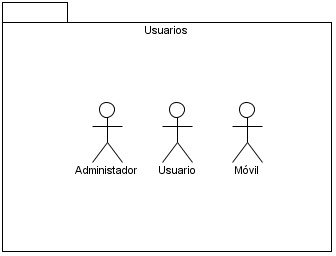
\includegraphics[width=0.7\textwidth]{ModeloComportamiento/imagenes/Actores.png}}
		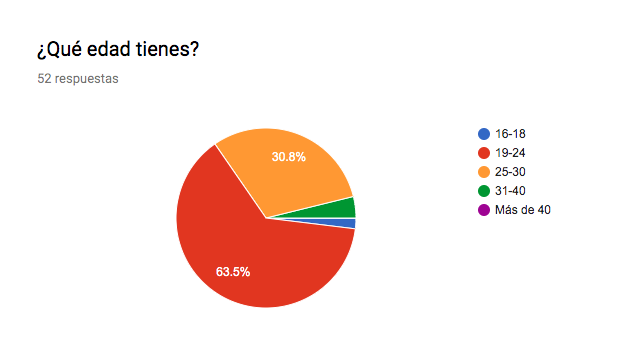
\includegraphics[width=0.85\textwidth]{DisenoEstructura/imagenes/Pregunta1}
		\caption{Pregunta1}
		\label{DE/FO/Pregunta1}
	\end{center}
\end{figure}

La primer pregunta fue para localizar un rango de edad del uso de la herramienta.Dentro de la encuesta se encontro que predominan las personas con una edad de 19 a los 24 años. Con un total de 63.5\% \\


\subsection{Género}

\begin{figure}[htbp!]
	\begin{center}
		%\fbox{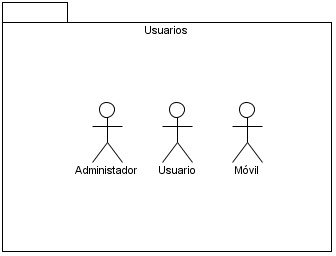
\includegraphics[width=0.7\textwidth]{ModeloComportamiento/imagenes/Actores.png}}
		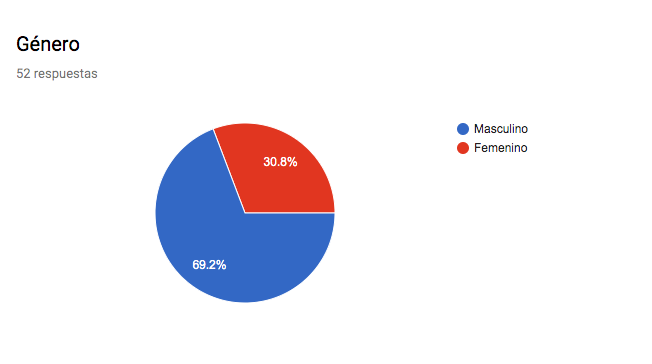
\includegraphics[width=0.85\textwidth]{DisenoEstructura/imagenes/Pregunta2}
		\caption{Pregunta2}
		\label{DE/FO/Pregunta2}
	\end{center}
\end{figure}

La pregunta género nos ayudo a determinar hacia que personas va mayormente dirigida nuestra herramienta. Arrojando como resultado que predomina el género masculino dentro de el mercado al que va dirigido nuestra apliación.\\

\subsection{¿Con que frecuencia utilizas automóvil? (Por semana)}

\begin{figure}[htbp!]
	\begin{center}
		%\fbox{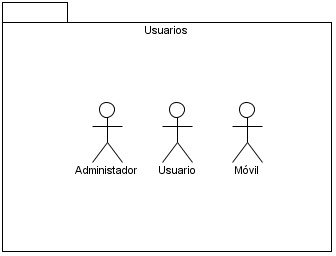
\includegraphics[width=0.7\textwidth]{ModeloComportamiento/imagenes/Actores.png}}
		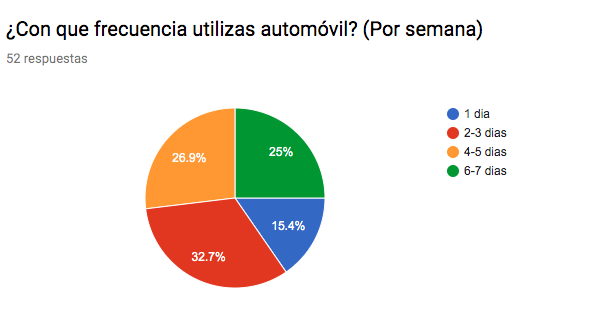
\includegraphics[width=0.7\textwidth]{DisenoEstructura/imagenes/Pregunta3}
		\caption{Pregunta3}
		\label{DE/FO/Pregunta3}
	\end{center}
\end{figure}

Uno de los puntos importantes es saber con que frecuencia viajan en automovil nuestros usuarios por ende los resultados a esta pregunta fueron satisfactorios quedando asi como primer lugar de 2-3 dias a la semana con un 32.7\% . \\

\subsection{Cuando Viajas en automóvil. Con mayor frecuencia ¿Eres?}

\begin{figure}[htbp!]
	\begin{center}
		%\fbox{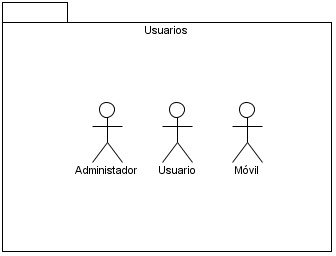
\includegraphics[width=0.7\textwidth]{ModeloComportamiento/imagenes/Actores.png}}
		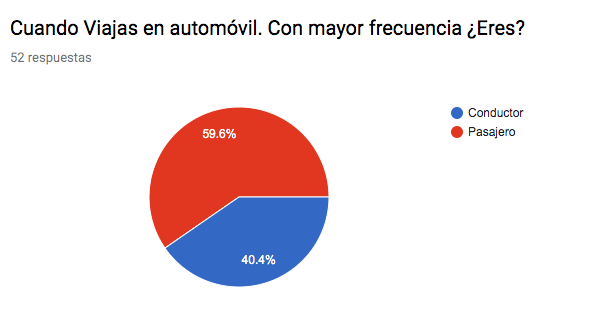
\includegraphics[width=0.85\textwidth]{DisenoEstructura/imagenes/Pregunta4}
		\caption{Pregunta4}
		\label{DE/FO/Pregunta4}
	\end{center}
\end{figure}

La mayoria de las ocasiones en las cuales se hace uso de del automovil no siempre se es conductor , como se muestra en los resultados arrojados por la encuesta formulada , dando un total de 59.6 \% a personas que son pasajeros durante el uso de un automovil.\\


\subsection{¿Cuentas con mas de un vehículo?}

\begin{figure}[htbp!]
	\begin{center}
		%\fbox{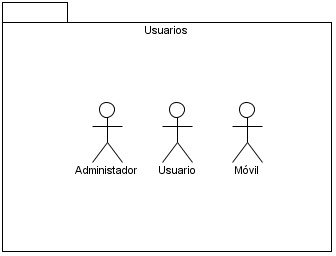
\includegraphics[width=0.7\textwidth]{ModeloComportamiento/imagenes/Actores.png}}
		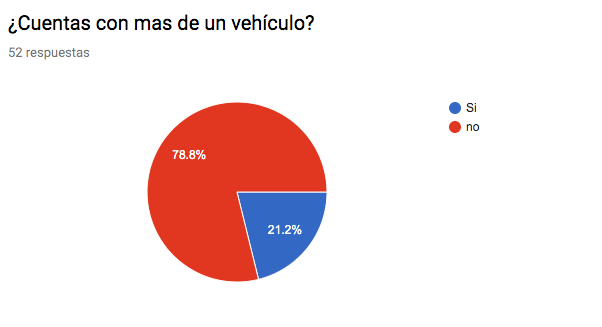
\includegraphics[width=0.85\textwidth]{DisenoEstructura/imagenes/Pregunta5}
		\caption{Pregunta5}
		\label{DE/FO/Pregunta5}
	\end{center}
\end{figure}

Para poder definir el numero de vehiculos a registrar dentro de la herramienta , se realizo el censo para saber si los usuarios cuentan con mas de un vehiculo , lo cual nos llevo a saber que existe un pequeña parte de usuarios que cuentan con mas de un vehiculo.\\

\subsection{¿Que marca es tu automóvil?}

\begin{figure}[htbp!]
	\begin{center}
		%\fbox{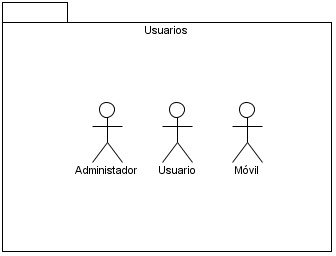
\includegraphics[width=0.7\textwidth]{ModeloComportamiento/imagenes/Actores.png}}
		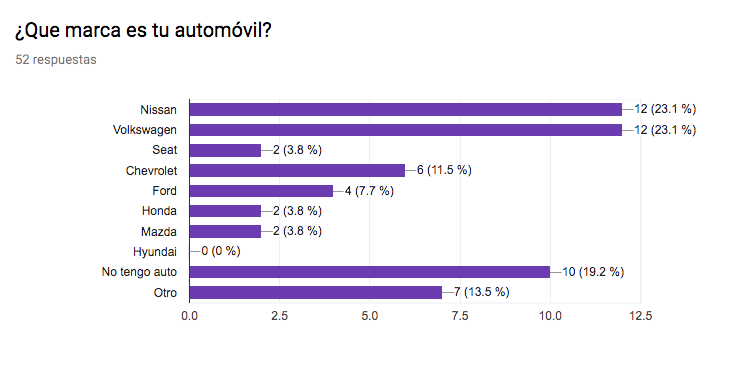
\includegraphics[width=0.85\textwidth]{DisenoEstructura/imagenes/Pregunta6}
		\caption{Pregunta6}
		\label{DE/FO/Pregunta6}
	\end{center}
\end{figure}

Para determinar hacia que marca de automovil vamos a estar enfocados se realizo el censo de las marcas mas encontradas dentro de nuestro mercado, quedando asi  Nissan y Volkswagen como las marcas con mas uso dentro de esta encuesta realizada.\\

\subsection{¿Que información conoces de tu automóvil?}

\begin{figure}[htbp!]
	\begin{center}
		%\fbox{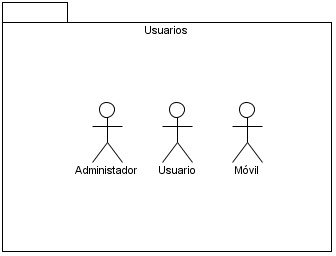
\includegraphics[width=0.7\textwidth]{ModeloComportamiento/imagenes/Actores.png}}
		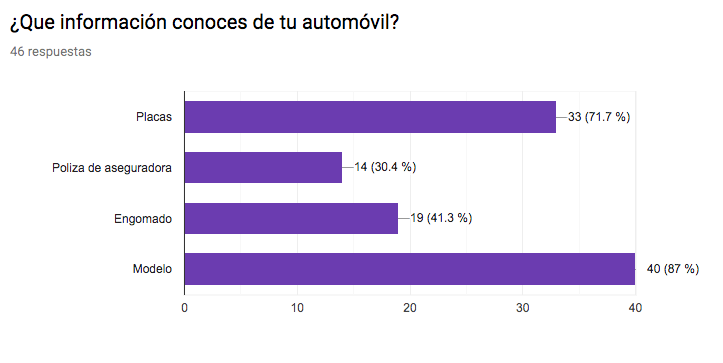
\includegraphics[width=0.85\textwidth]{DisenoEstructura/imagenes/Pregunta7}
		\caption{Pregunta7}
		\label{DE/FO/Pregunta7}
	\end{center}
\end{figure}

Para determinar la información a solicitar dentro de la aplicación se realizo la pregunta anterior , por lo cual se puede observar que el modelo del automovil es lo que con mas frecuencia identifican los usuario , despues identifican con mayor facilidad las placas , despues el engomado correspodiente a dicho automovil , por ultimo pero no menos importante , la poliza aseguradora.\\

\subsection{¿Has participado o estado presente en algún choque automovilístico?}

\begin{figure}[htbp!]
	\begin{center}
		%\fbox{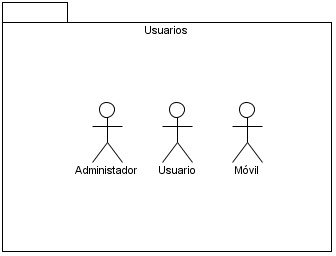
\includegraphics[width=0.7\textwidth]{ModeloComportamiento/imagenes/Actores.png}}
		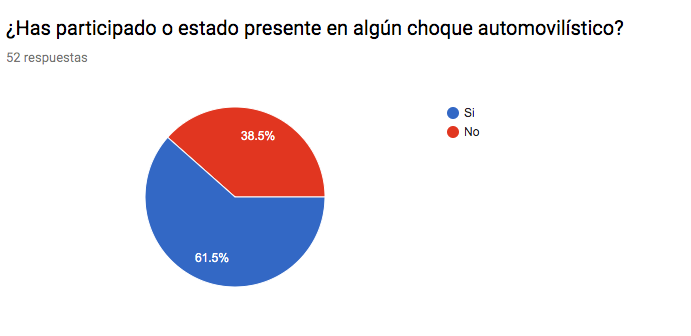
\includegraphics[width=0.85\textwidth]{DisenoEstructura/imagenes/Pregunta8}
		\caption{Pregunta8}
		\label{DE/FO/Pregunta8}
	\end{center}
\end{figure}

Para poder sustentar la frecuencia con la que ocuren los accidentes automovilísticos , se realizo la pregunta anterior , la cual arrojo como resultado que un 61.5\% si ha participado o estado presente durante un choque automovilístico. \\

\subsection{En caso de haber seleccionado si . ¿Sufriste algún tipo de lesion durante el percance?}

\begin{figure}[htbp!]
	\begin{center}
		%\fbox{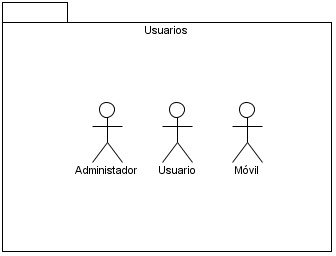
\includegraphics[width=0.7\textwidth]{ModeloComportamiento/imagenes/Actores.png}}
		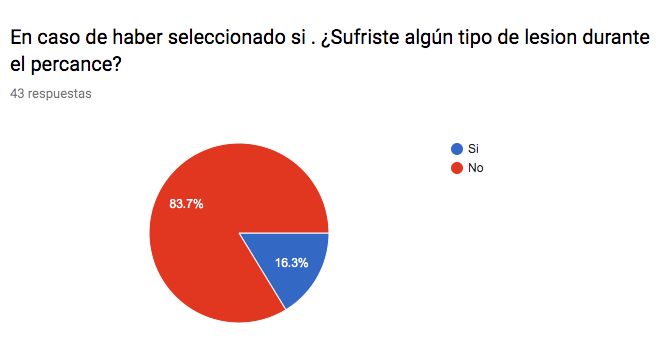
\includegraphics[width=0.7\textwidth]{DisenoEstructura/imagenes/Pregunta9}
		\caption{Pregunta9}
		\label{DE/FO/Pregunta9}
	\end{center}
\end{figure}

Las lesiones durante los percances puede relacionarse a gravedad de la lesion , por ende se realizo la anterior pregunta dando asi como resultado un total de 16.3\%  de personas que han tenido una lesion durante el suceso.\\

\subsection{¿Que servicio de seguro social tienes?}

\begin{figure}[htbp!]
	\begin{center}
		%\fbox{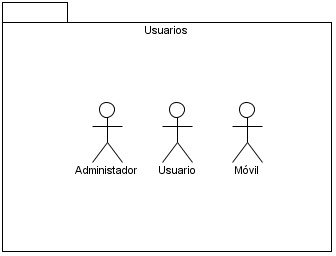
\includegraphics[width=0.7\textwidth]{ModeloComportamiento/imagenes/Actores.png}}
		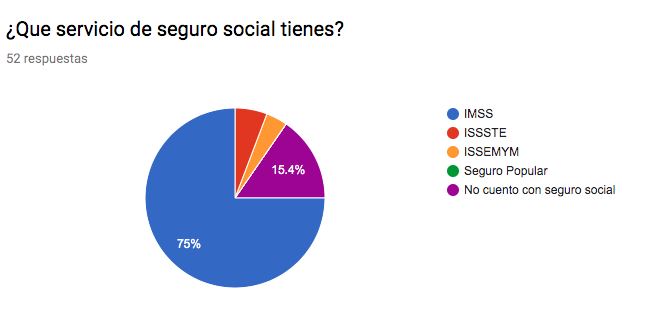
\includegraphics[width=0.85\textwidth]{DisenoEstructura/imagenes/Pregunta10}
		\caption{Pregunta10}
		\label{DE/FO/Pregunta10}
	\end{center}
\end{figure}

El seguro social es sumamente importante para la atencióon medica inmediata de nuestros usuarios , gracias a la pregunta realizada anteriormente se ha recolectado que el Instituto Mexicano Del Seguro Social tiene el mayor indice de derechohabientes con un porcentaje del 75\%  quedando así como el servicio mayormente utilizado por nuestros usuarios.  

\subsection{En caso de tener automóvil. ¿Cuentas con aseguradora vehicular?}

\begin{figure}[htbp!]
	\begin{center}
		%\fbox{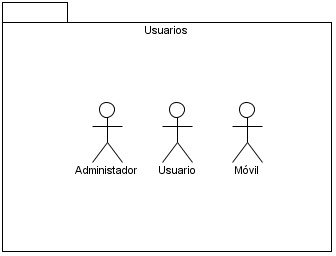
\includegraphics[width=0.7\textwidth]{ModeloComportamiento/imagenes/Actores.png}}
		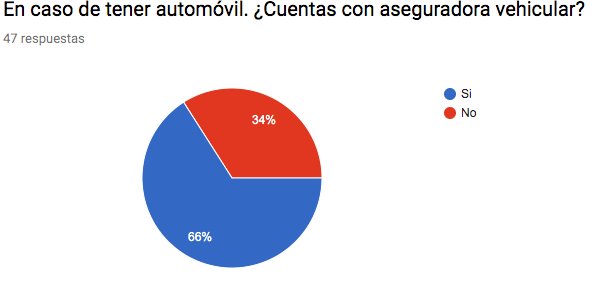
\includegraphics[width=0.85\textwidth]{DisenoEstructura/imagenes/Pregunta11}
		\caption{Pregunta11}
		\label{DE/FO/Pregunta11}
	\end{center}
\end{figure}

Otra parte importante a destacar dentro de la aplicación es saber cuantas usuarios cuenta con aseguradora vehicular. Por lo tanto la encuesta arrojo un porcentaje del 66\% de usuarios que cuentan con aseguradora vehicular , lo que vuelve un punto importante para la operabilidad de la aplicación.\\

\subsection{¿Has tenido decesos de algún familiar, amigo o conocido ; Derivado de un accidente automovilístico?}

\begin{figure}[htbp!]
	\begin{center}
		%\fbox{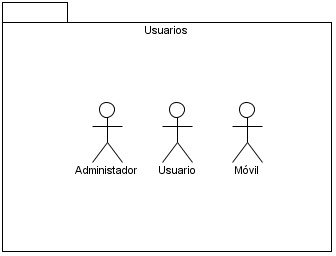
\includegraphics[width=0.7\textwidth]{ModeloComportamiento/imagenes/Actores.png}}
		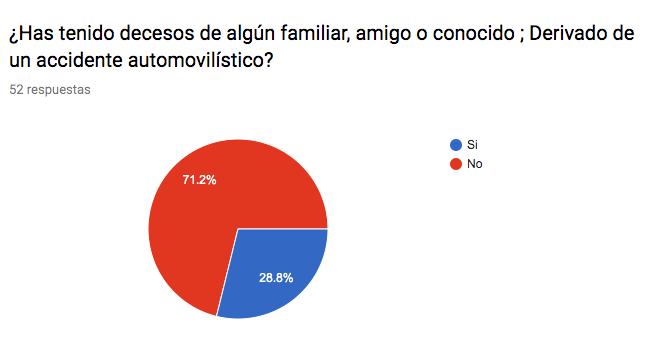
\includegraphics[width=0.85\textwidth]{DisenoEstructura/imagenes/Pregunta12}
		\caption{Pregunta12}
		\label{DE/FO/Pregunta12}
	\end{center}
\end{figure}

El sustento de la aplicación se centra en los decesos automovilisticos que han ocurrido por ende se realizo la pregunta anterior , en la cual podemos destacar que desafortunadamente un 28.8\% han tenido decesos durante un choque automovilistico.\\

\subsection{¿Crees que la falta de notificación inmediata durante un choque automovilístico influye al salvar una vida?}

\begin{figure}[htbp!]
	\begin{center}
		%\fbox{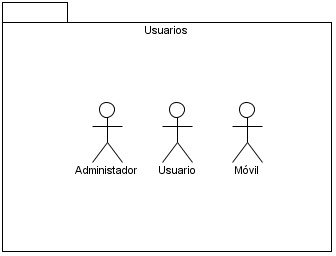
\includegraphics[width=0.7\textwidth]{ModeloComportamiento/imagenes/Actores.png}}
		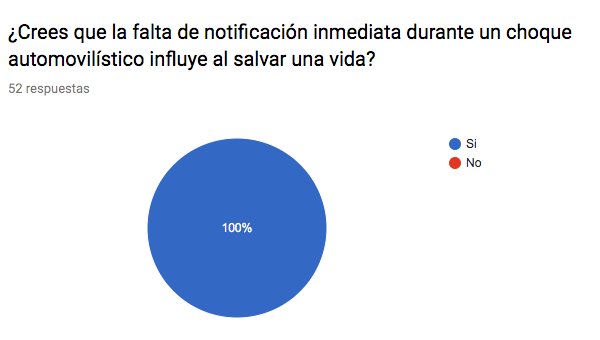
\includegraphics[width=0.6\textwidth]{DisenoEstructura/imagenes/Pregunta13}
		\caption{Pregunta13}
		\label{DE/FO/Pregunta13}
	\end{center}
\end{figure}

El punto clave y el por que del desarrollo se centra en la pregunta anterior .La encuesta ha arrojado un porcentaje unanime por lo cual de llego a la conclusión de que la falta de notificación inmediata durante un choque automovilístico influye al salvar vidas.\\

\subsection{En caso de hospitalización ¿Que datos consideras mas importantes?}

\begin{figure}[htbp!]
	\begin{center}
		%\fbox{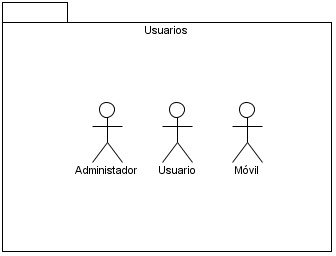
\includegraphics[width=0.7\textwidth]{ModeloComportamiento/imagenes/Actores.png}}
		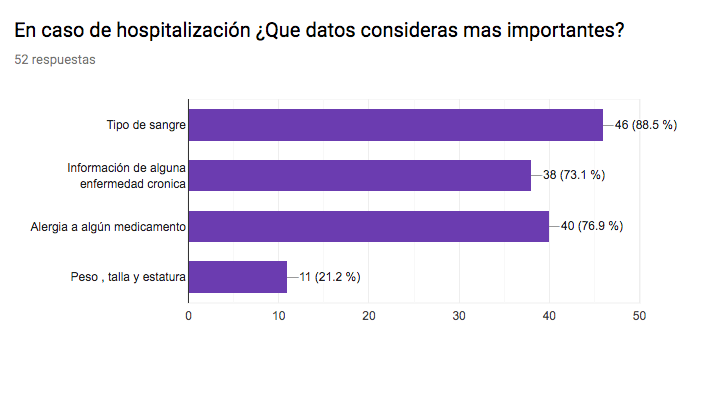
\includegraphics[width=0.85\textwidth]{DisenoEstructura/imagenes/Pregunta14}
		\caption{Pregunta14}
		\label{DE/FO/Pregunta14}
	\end{center}
\end{figure}

En caso de llegar a una hospitalización de cualquier indole es importante considerar varios factores por ello se realizo la pregunta anterior en la cual los usuarios determinaron que el tipo de sangre es el factor mas importante durante una hospitalización seguido de cualquier tipo de alergia a medicamentos y por utlimo información sobre enfermedades cronicas. \\

\subsection{¿Cuentas con alguna aplicación móvil que detecte cuando has tenido algún choque automovilístico?}

\begin{figure}[htbp!]
	\begin{center}
		%\fbox{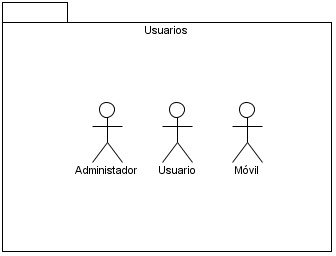
\includegraphics[width=0.7\textwidth]{ModeloComportamiento/imagenes/Actores.png}}
		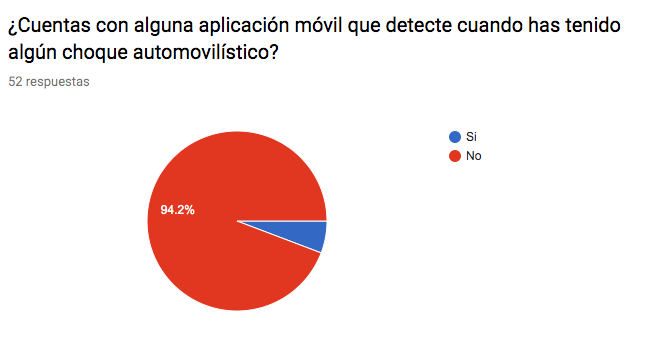
\includegraphics[width=0.65\textwidth]{DisenoEstructura/imagenes/Pregunta15}
		\caption{Pregunta15}
		\label{DE/FO/Pregunta15}
	\end{center}
\end{figure}

La competencia en el mercado de acuerdo a la encuesta realizada la marca como casi nula , podemos deducir eso por los resultados arrojados a esta pregunta que cuenta con un porcentaje total del 94.2\% de que no cuenta con una aplicación movil que notifique cuando ha habido algún choque automivílistio.\\

\subsection{Si cuentas con la aplicación móvil ¿Cual fue el costo?}

\begin{figure}[htbp!]
	\begin{center}
		%\fbox{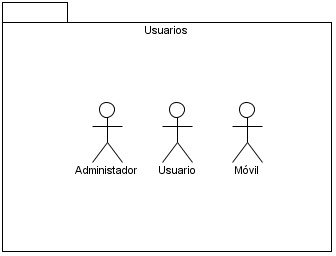
\includegraphics[width=0.7\textwidth]{ModeloComportamiento/imagenes/Actores.png}}
		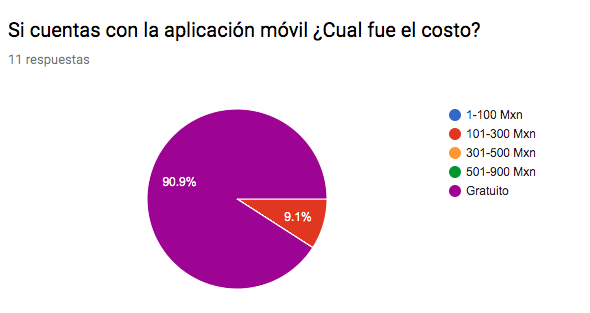
\includegraphics[width=0.85\textwidth]{DisenoEstructura/imagenes/Pregunta16}
		\caption{Pregunta16}
		\label{DE/FO/Pregunta16}
	\end{center}
\end{figure}

Por motivo a la pregunta anterior podemos observar que la aplicación movil puede entrar en un gran parte del mecardo de una forma gratuita.

\subsection{Una aplicación que notifique a contactos de emergencia o familiares durante una colisión automovilística ¿La utilizarias?}

\begin{figure}[htbp!]
	\begin{center}
		%\fbox{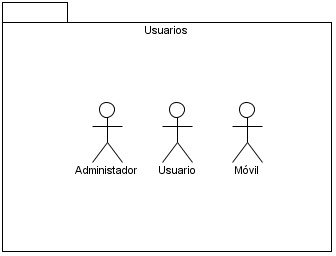
\includegraphics[width=0.7\textwidth]{ModeloComportamiento/imagenes/Actores.png}}
		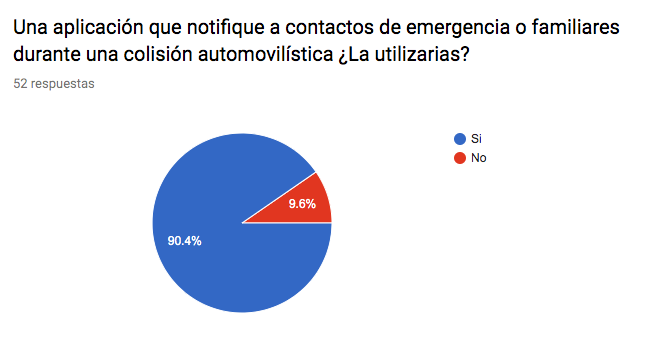
\includegraphics[width=0.65\textwidth]{DisenoEstructura/imagenes/Pregunta17}
		\caption{Pregunta17}
		\label{DE/FO/Pregunta17}
	\end{center}
\end{figure}

La pregunta anterior se realizo para poder deducir el auge que puede tener la aplicación movil In-Help , como se nota en la pregunta anterior el indice de respuesta a el uso de la aplicación movil fue alto . Gracias a ello podemos intentar satisfacer al mercado con las caracteristicas de la aplicación movil anteriormente mencionada.

\subsection{¿Estarias dispuesto a pagar por una aplicación que notifique a los cuerpos medicos cuando seas participe de un choque automovilístico?}

\begin{figure}[htbp!]
	\begin{center}
		%\fbox{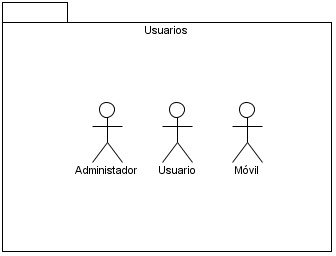
\includegraphics[width=0.7\textwidth]{ModeloComportamiento/imagenes/Actores.png}}
		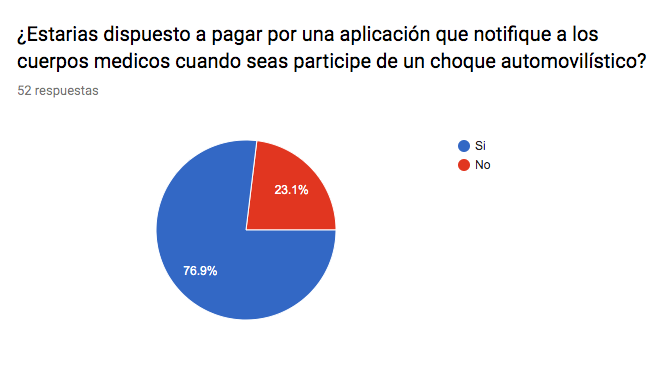
\includegraphics[width=0.85\textwidth]{DisenoEstructura/imagenes/Pregunta18}
		\caption{Pregunta18}
		\label{DE/FO/Pregunta18}
	\end{center}
\end{figure}

Uno de los puntos que cabe destacar dentro de la aplicación es saber cuantas personas adquiririan In-Help por cualquier tipo de costo . Para ello se realizo la pregunta anterior la que arrojo un porcentaje total de 76.9\% que pagarian por la utilización de la aplicación.

\subsection{¿Que marca de smartphone utilizas?}

\begin{figure}[htbp!]
	\begin{center}
		%\fbox{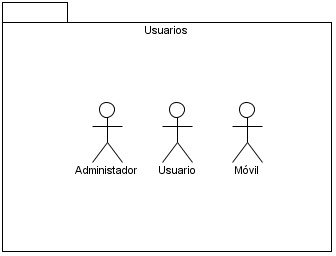
\includegraphics[width=0.7\textwidth]{ModeloComportamiento/imagenes/Actores.png}}
		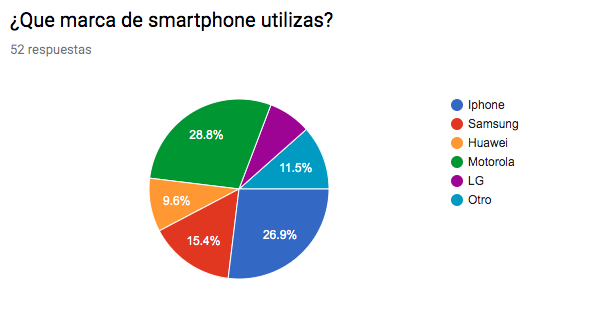
\includegraphics[width=0.65\textwidth]{DisenoEstructura/imagenes/Pregunta19}
		\caption{Pregunta19}
		\label{DE/FO/Pregunta19}
	\end{center}
\end{figure}

Los smartphones con el paso del tiempo han ido evolucionando y con ello se han creado una gran cantidad de dispositivos moviles . Para saber cual es la marca mas popular y mas utilizada por los usuarios , se realizó la pregunta anterior , con la cual se llego a la conclusión de que motorola es la marca de smarthphone con mayor auge con un porcentaje total de 28.8\% . \\

\subsection{¿Que tipo de sistema operativo utiliza tu dispositivo móvil?}

\begin{figure}[htbp!]
	\begin{center}
		%\fbox{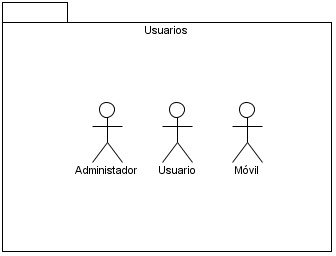
\includegraphics[width=0.7\textwidth]{ModeloComportamiento/imagenes/Actores.png}}
		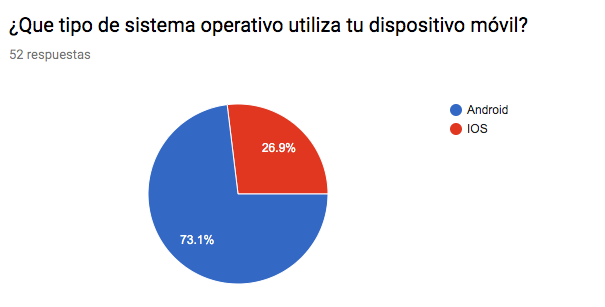
\includegraphics[width=0.85\textwidth]{DisenoEstructura/imagenes/Pregunta20}
		\caption{Pregunta20}
		\label{DE/FO/Pregunta20}
	\end{center}
\end{figure}

Para determinar el sistema operativo por el cual se va a trabajar se realizo esta pregunta. Como se muestra en la encuesta y podemos observar en la pregunta anterior la mayor parte de los smarthphones utilizados contienen un sistema operativo Android , por lo cual se llego a la conclusión de Android es el sistema operativo como mejor iteroperabilidad para la realización de In-Help.\\

\subsection{¿Te serviria una aplicación donde estuviera concentrada la información de tu vehículo , tales como números de aseguradora , números de emergencia y familiares de emergencia?}

\begin{figure}[htbp!]
	\begin{center}
		%\fbox{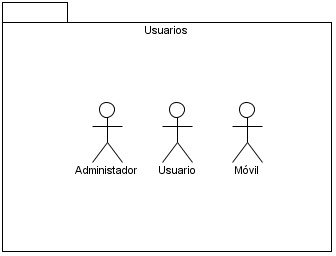
\includegraphics[width=0.7\textwidth]{ModeloComportamiento/imagenes/Actores.png}}
		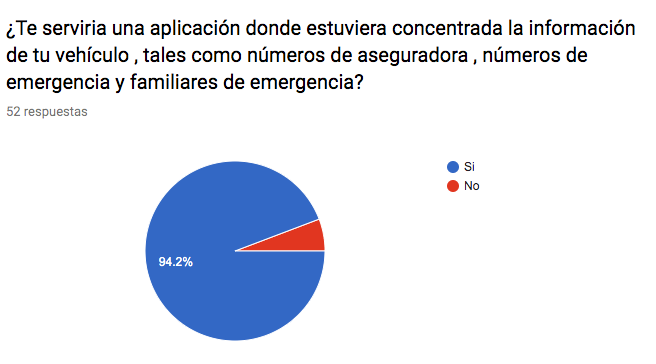
\includegraphics[width=0.85\textwidth]{DisenoEstructura/imagenes/Pregunta21}
		\caption{Pregunta21}
		\label{DE/FO/Pregunta21}
	\end{center}
\end{figure}

Como última pregunta se intenta saber si la información que despues de la encuesta sera introducida en la aplicación es útil para los usuarios que hagan uso de In-Help.\\





